\section{129 --- Sum Root to Leaf Numbers}
Given a binary tree containing digits from 0--9 only, each root-to-leaf path could represent a number.

An example is the root-to-leaf path $1\longrightarrow 2\longrightarrow 3$ which represents the number $123$.

Find the total sum of all root-to-leaf numbers.

\paragraph{Note:}
\begin{itemize}
    \item A leaf is a node with no children.
\end{itemize}


\paragraph{Example:}

\begin{flushleft}


\textbf{Input}: 
\begin{figure}[H]
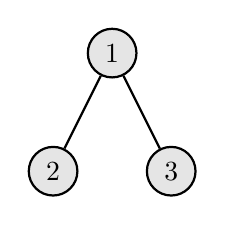
\begin{tikzpicture}
[every node/.style={draw, circle, minimum size=6mm, fill=gray!20!},  node distance=8mm,  thick]
\node{1}
child{node{2}}
child{node{3}};
\end{tikzpicture}
\end{figure}


\textbf{Output}: 25

\textbf{Explanation}:

The root-to-leaf path $1\longrightarrow 2$ represents the number $12$.

The root-to-leaf path $1\longleftrightarrow 3$ represents the number $13$.

Therefore, sum is $12 + 13 = 25$.
\end{flushleft}


\paragraph{Example 2:}

\begin{flushleft}
\begin{figure}[H]
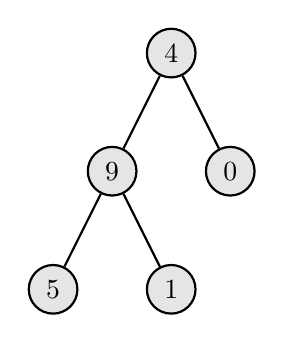
\begin{tikzpicture}
[every node/.style={draw, circle, minimum size=6mm, fill=gray!20!},  node distance=8mm,  thick]
\node{4}
child{node{9} child{node{5}} child{node{1}}}
child{node{0}};
\end{tikzpicture}
\end{figure}

\textbf{Output}: $1026$

\textbf{Explanation}:

The root-to-leaf path $ 4\longrightarrow9\longrightarrow5 $ represents the number $ 495 $.

The root-to-leaf path $4\longrightarrow 9\longrightarrow 1$ represents the number $ 491 $.

The root-to-leaf path $4\longrightarrow 0$ represents the number $ 40 $.

Therefore, sum is $495 + 491 + 40 = 1026$.
\end{flushleft}